\utsubsection{Inter OpenBTS Handover}{Thomas Waldecker}\label{sec:interbts}

Dieser Abschnitt beschreibt die theoretische Umsetzung eines Inter OpenBTS Hand\-overs. Als Vorraussetzung wird angenommen das eine OpenBTS Basisstation seine Benachbarten OpenBTS Basisstationen kennt. Alle OpenBTS sind mit einem Asterisk Server verbunden. Die Basisstationen können sich untereinander per IP erreichen. Ist jetzt ein Anruf aktiv auf einer Mobilstation und entscheidet die Basisstation das sie einen Handover durchführen möchte, führen die beiden Basisstationen einen peer-to-peer Handover durch, wobei die aktuelle Basisstation die Masterbasisstation ist.

\begin{figure}[htbp]
	\centering
		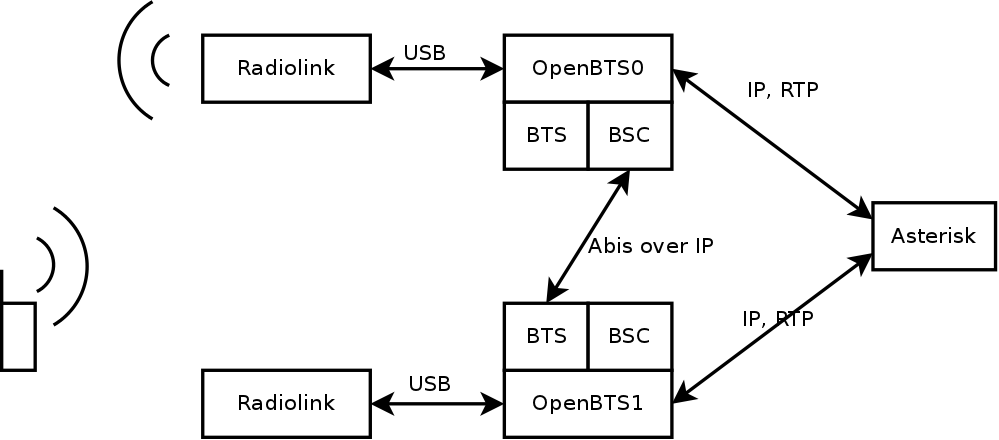
\includegraphics[width=0.9\textwidth]{img/inter_openbts}
	\caption{Kommunikation zwischen den Komponenten}
	\label{fig:interopenbts_komm}
\end{figure}

Sieht man die aktuelle Basisstation als BSC mit BTS und die neue OpenBTS Basisstation als reine BTS an, so wäre das Handoverszenario vergleichbar mit einem Intra BSC Handover.

Eine Weiterleitung des Sprachkanals kann entweder im Asterisk erfolgen oder von der origin OpenBTS zur neuen OpenBTS weitergeleitet werden. 
